\documentclass[12pt,a4paper]{article}

\usepackage{fancyhdr}
\usepackage{graphicx}
\usepackage{placeins}
\usepackage{adjustbox}


\begin{document}

\pagestyle{fancy}
\fancyhf{}
\chead{Short summary report}

\begin{table}[t]
\centering
\caption {rnaQUAST metrics for assembled transcripts. In each row the best values are indicated with \textbf{bold}. For the transcript metrics (rows 4, 5, 6, 9, 13, 26, 27, 28) we highlighted the best \textbf{relative} values i.e. divided by the total number of transcripts in the corresponding assembly.}
\begin{adjustbox}{width=1\textwidth}
\small
\begin{tabular}{|l*{11}{|r}|}
\hline
\textbf{METRICS/TRANSCRIPTS}                            & \textbf{Trinity}       & \textbf{Trans-ABySS}   & \textbf{Oases}         & \textbf{SOAPdenovo-Trans} & \textbf{IDBA-Tran}     & \textbf{Bridger}       & \textbf{BinPacker}     & \textbf{Shannon}       & \textbf{rnaSPAdes}     & \textbf{SPAdes}        \\ \hline\hline
\multicolumn{11}{l}{\bf DATABASE METRICS}                                                 \\ \hline
Genes                                                   & 3119                   & 3119                   & 3119                   & 3119                   & 3119                   & 3119                   & 3119                   & 3119                   & 3119                   & 3119                   \\
Avg. number of exons per isoform                        & 6.99                   & 6.99                   & 6.99                   & 6.99                   & 6.99                   & 6.99                   & 6.99                   & 6.99                   & 6.99                   & 6.99                   \\ \hline
\multicolumn{11}{l}{\bf BASIC TRANSCRIPTS METRICS}                                        \\ \hline
Transcripts                                             & 13484                  & 25272                  & 46469                  & 14965                  & 12151                  & 10457                  & 13415                  & 7255                   & 11766                  & 10537                  \\
Transcripts $>$ 500 bp                                  & \textbf{10717}         & 11460                  & 34981                  & 6270                   & 5642                   & 7180                   & 9858                   & 3729                   & 9116                   & 4309                   \\
Transcripts $>$ 1000 bp                                 & \textbf{8451}          & 6703                   & 28143                  & 4263                   & 2740                   & 5167                   & 7424                   & 2341                   & 6053                   & 2623                   \\ \hline
\multicolumn{11}{l}{\bf ALIGNMENT METRICS}                                                \\ \hline
Aligned                                                 & 13454                  & 25150                  & 46049                  & 14792                  & \textbf{12134}         & 10307                  & 13252                  & 7196                   & 11744                  & 10503                  \\
Uniquely aligned                                        & 13214                  & 24896                  & 41196                  & 14692                  & 12099                  & 9537                   & 12174                  & 7035                   & 11306                  & 10347                  \\
Multiply aligned                                        & 12                     & 39                     & 48                     & 18                     & 11                     & 7                      & 10                     & 7                      & 7                      & 87                     \\
Unaligned                                               & 30                     & 122                    & 420                    & 173                    & \textbf{17}            & 150                    & 163                    & 59                     & 22                     & 34                     \\ \hline
\multicolumn{11}{l}{\bf ALIGNMENT METRICS FOR NON-MISASSEMBLED TRANSCRIPTS}               \\ \hline
Avg. aligned fraction                                   & 0.989                  & 0.994                  & 0.959                  & 0.994                  & \textbf{0.998}         & 0.983                  & 0.981                  & 0.996                  & 0.968                  & 0.995                  \\
Avg. alignment length                                   & \textbf{2261.332}      & 939.312                & 2090.55                & 1009.08                & 859.966                & 1581.299               & 1755.155               & 1061.013               & 1649.147               & 979.981                \\
Avg. mismatches per transcript                          & 1.231                  & 0.459                  & 2.105                  & 0.308                  & \textbf{0.096}         & 1.652                  & 1.849                  & 0.394                  & 1.82                   & 0.215                  \\ \hline
\multicolumn{11}{l}{\bf ALIGNMENT METRICS FOR MISASSEMBLED (CHIMERIC) TRANSCRIPTS}          \\ \hline
Misassemblies                                           & 139                    & 117                    & 4094                   & 49                     & \textbf{8}             & 533                    & 785                    & 66                     & 351                    & 50                     \\ \hline
\multicolumn{11}{l}{\bf ASSEMBLY COMPLETENESS (SENSITIVITY)}                              \\ \hline
Database coverage                                       & 0.461                  & 0.535                  & \textbf{0.592}         & 0.406                  & 0.382                  & 0.346                  & 0.372                  & 0.189                  & 0.431                  & 0.367                  \\
50\%-assembled genes                                    & 2478                   & \textbf{2680}          & 2623                   & 2365                   & 2494                   & 2247                   & 2300                   & 1441                   & 2606                   & 2537                   \\
95\%-assembled genes                                    & 1915                   & \textbf{2074}          & 1865                   & 1380                   & 570                    & 1353                   & 1402                   & 854                    & 1760                   & 1566                   \\
50\%-covered genes                                      & 2644                   & \textbf{2903}          & 2812                   & 2719                   & 2733                   & 2427                   & 2480                   & 1621                   & 2686                   & 2624                   \\
95\%-covered genes                                      & 2096                   & \textbf{2485}          & 2052                   & 1755                   & 1158                   & 1527                   & 1579                   & 954                    & 2025                   & 1772                   \\
50\%-assembled isoforms                                 & 4654                   & 5992                   & \textbf{6106}          & 3630                   & 3896                   & 3362                   & 3701                   & 1920                   & 4557                   & 3668                   \\
95\%-assembled isoforms                                 & 2898                   & 2877                   & \textbf{2995}          & 1679                   & 577                    & 1570                   & 1660                   & 1056                   & 2220                   & 1625                   \\
50\%-covered isoforms                                   & 5003                   & \textbf{6966}          & 6780                   & 4399                   & 4760                   & 3725                   & 4086                   & 2183                   & 4848                   & 4054                   \\
95\%-covered isoforms                                   & 3254                   & \textbf{3785}          & 3525                   & 2145                   & 1203                   & 1786                   & 1907                   & 1181                   & 2596                   & 1865                   \\
Mean isoform coverage                                   & \textbf{0.806}         & 0.674                  & 0.737                  & 0.606                  & 0.591                  & 0.655                  & 0.659                  & 0.658                  & 0.717                  & 0.576                  \\
Mean isoform assembly                                   & \textbf{0.759}         & 0.602                  & 0.682                  & 0.531                  & 0.512                  & 0.61                   & 0.614                  & 0.599                  & 0.678                  & 0.538                  \\ \hline
\multicolumn{11}{l}{\bf GeneMarkS-T METRICS}                                              \\ \hline
Predicted genes                                         & 6829                   & 8600                   & \textbf{21274}         & 3567                   & 4599                   & 4400                   & 6344                   & 2598                   & 6088                   & 2863                   \\ \hline
\multicolumn{11}{l}{\bf ASSEMBLY SPECIFICITY}                                             \\ \hline
50\%-matched                                            & 12797                  & 24508                  & 38562                  & 14251                  & \textbf{12072}         & 9287                   & 11761                  & 7005                   & 10955                  & 10295                  \\
95\%-matched                                            & 5462                   & 16312                  & 16512                  & 9194                   & \textbf{8280}          & 4556                   & 5451                   & 4606                   & 5031                   & 7030                   \\
Unannotated                                             & 96                     & 82                     & 585                    & 24                     & \textbf{6}             & 34                     & 62                     & 8                      & 37                     & 44                     \\
Mean fraction of transcript matched                     & 0.864                  & 0.927                  & 0.84                   & 0.907                  & \textbf{0.934}         & 0.884                  & 0.87                   & 0.931                  & 0.875                  & 0.919                  \\ \hline
\end{tabular}
\end{adjustbox}
\end{table}

\FloatBarrier
\clearpage
\lfoot{generated by rnaQUAST}

\begin{figure}[t]
\centering
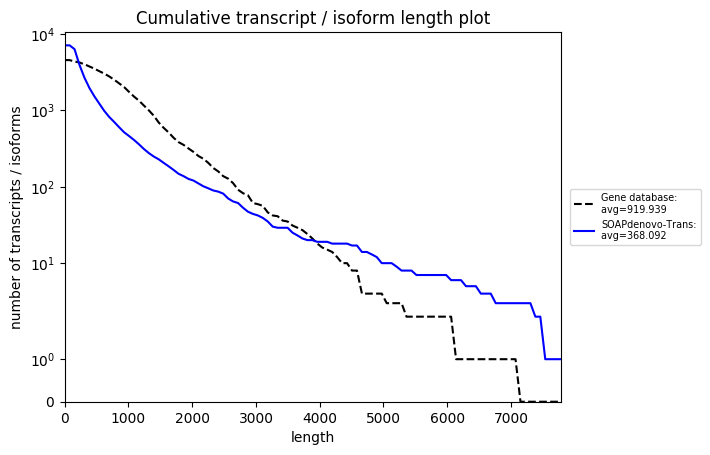
\includegraphics[width = \linewidth]{/mnt/dessertlocal/projects/transcriptome_assembly/review/evaluation/rna-quast/hsa_flux/comparison_output/transcript_length.png}
\caption{Plot showing cumulative transcript length distribution. Each point represents the number of transcripts in the assembly with the corresponding length or longer; black dashed line corresponds to the database isoforms; the plot is given in logarithmic scale.}
\end{figure}
\FloatBarrier
\clearpage


\begin{figure}[t]
\centering
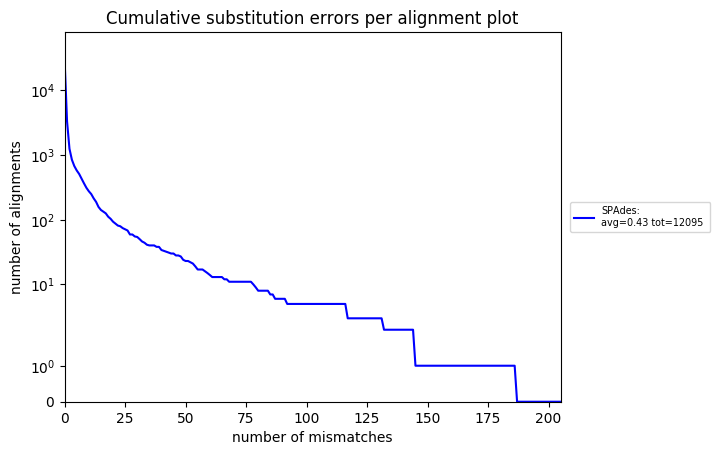
\includegraphics[width = \linewidth]{/mnt/dessertlocal/projects/transcriptome_assembly/review/evaluation/rna-quast/hsa_flux/comparison_output/mismatch_rate.png}
\caption{Plot showing cumulative substitution errors per alignment distribution. Each point represents the number of alignments with the corresponding number of mismatches or greater; the plot is given in logarithmic scale.}
\end{figure}
\FloatBarrier
\clearpage


\begin{figure}[t]
\centering
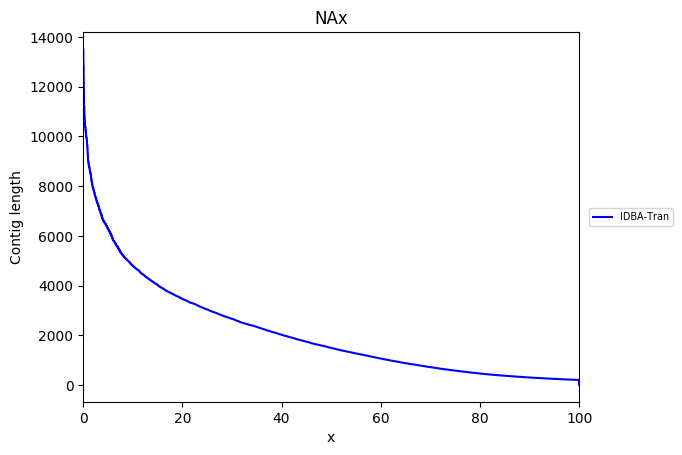
\includegraphics[width = \linewidth]{/mnt/dessertlocal/projects/transcriptome_assembly/review/evaluation/rna-quast/hsa_flux/comparison_output/NAx.png}
\caption{Nx plot for transcripts. Nx is a maximal number $N$, such that the total length of all transcripts longer than $N$ bp is at least $x\%$ of the total length of all transcripts.}
\end{figure}
\FloatBarrier
\clearpage


\begin{figure}[t]
\centering
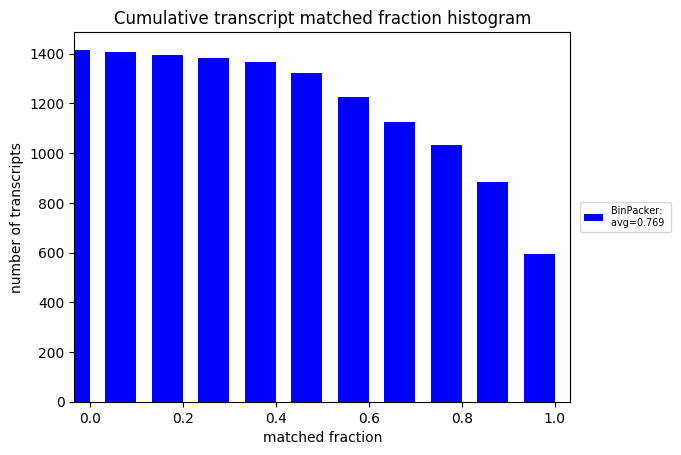
\includegraphics[width = \linewidth]{/mnt/dessertlocal/projects/transcriptome_assembly/review/evaluation/rna-quast/hsa_flux/comparison_output/x-matched.png}
\caption{Plot showing cumulative transcript match histogram. Each bar represents the number of transcripts with matched fraction equal to or greater than the value on $x$ axis; transcript matched fraction is calculated as the number of its bases covering an isoform divided by the transcript length.}
\end{figure}
\FloatBarrier
\clearpage


\begin{figure}[t]
\centering
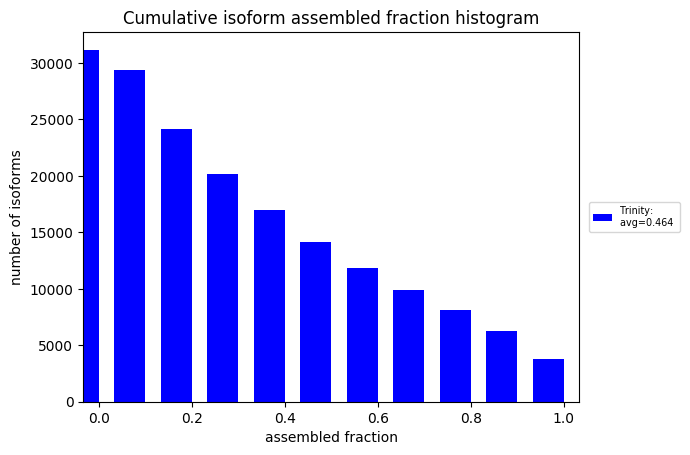
\includegraphics[width = \linewidth]{/mnt/dessertlocal/projects/transcriptome_assembly/review/evaluation/rna-quast/hsa_flux/comparison_output/x-assembled.png}
\caption{Plot showing cumulative isoform assembly histogram. Each bar represents the number of isoforms with assembled fraction equal to or greater than the value on $x$ axis; isoform assembled fraction is calculated as the maximum number of captured by single assembled transcript bases divided by the total isoform length.}
\end{figure}
\FloatBarrier
\clearpage


\begin{figure}[t]
\centering
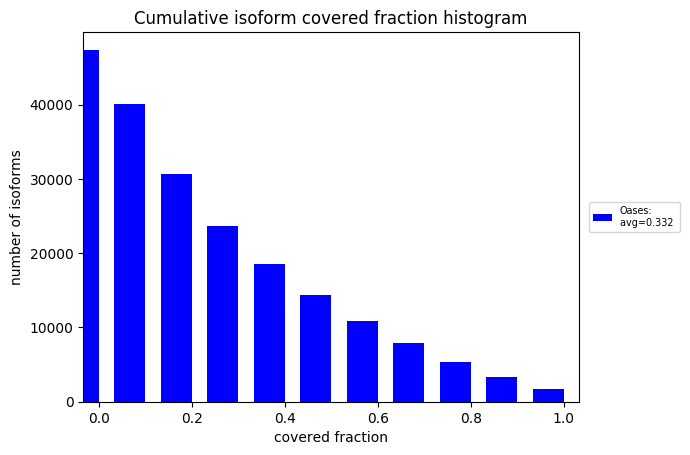
\includegraphics[width = \linewidth]{/mnt/dessertlocal/projects/transcriptome_assembly/review/evaluation/rna-quast/hsa_flux/comparison_output/x-covered.png}
\caption{Plot showing cumulative isoform coverage histogram. Each bar represents the number of isoforms with covered fraction equal to or greater than the value on $x$ axis; isoform covered fraction is calculated as the number of covered bases (by all transcripts in the assembly) divided by the total isoform length.}
\end{figure}
\FloatBarrier
\clearpage


\end{document}
